\documentclass[12pt,letterpaper,oneside,reqno]{amsart}
\usepackage{amsfonts}
\usepackage{amsmath}
\usepackage{amssymb}
\usepackage{amsthm}
\usepackage{float}
\usepackage{mathrsfs}
\usepackage{colonequals}
\usepackage[font=small,labelfont=bf]{caption}
\usepackage[left=1in,right=1in,bottom=1in,top=1in]{geometry}
\usepackage[pdfpagelabels,hyperindex,colorlinks=true,linkcolor=blue,urlcolor=magenta,citecolor=green]{hyperref}
\usepackage{graphicx}
\usepackage{spverbatim}
\linespread{1.7}
\emergencystretch=1em

\newcommand \anglePower [2]{\langle #1 \rangle \sp{#2}}
\newcommand \bernoulli [2][B] {{#1}\sb{#2}}
\newcommand \curvePower [2]{\{#1\}\sp{#2}}
\newcommand \coeffA [3][A] {{\mathbf{#1}} \sb{#2,#3}}
\newcommand \polynomialP [4][P]{{\mathbf{#1}}\sp{#2} \sb{#3}(#4)}

% ordinary derivatives
\newcommand \derivative [2] {\frac{d}{d #2} #1}                              % 1 - function; 2 - variable;
\newcommand \pderivative [2] {\frac{\partial #1}{\partial #2}}               % 1 - function; 2 - variable;
\newcommand \qderivative [1] {D_{q} #1}                                      % 1 - function
\newcommand \nqderivative [1] {D_{n,q} #1}                                   % 1 - function
\newcommand \qpowerDerivative [1] {\mathcal{D}_q #1}                         % 1 - function;
\newcommand \finiteDifference [1] {\Delta #1}                                % 1 - function;
\newcommand \pTsDerivative [2] {\frac{\partial #1}{\Delta #2}}               % 1 - function; 2 - variable;

% high order derivatives
\newcommand \derivativeHO [3] {\frac{d^{#3}}{d {#2}^{#3}} #1}                % 1 - function; 2 - variable; 3 - order
\newcommand \pderivativeHO [3]{\frac{\partial^{#3}}{\partial {#2}^{#3}} #1}
\newcommand \qderivativeHO [2] {D_{q}^{#2} #1}                               % 1 - function; 2 - order
\newcommand \qpowerDerivativeHO [2] {\mathcal{D}_{q}^{#2} #1}                % 1 - function; 2 - order
\newcommand \finiteDifferenceHO [2] {\Delta^{#2} #1}                         % 1 - function; 2 - order
\newcommand \pTsDerivativeHO [3] {\frac{\partial^{#3}}{\Delta {#2}^{#3}} #1} % 1 - function; 2 - variable;

\newtheorem{thm}{Theorem}[section]
\newtheorem{cor}[thm]{Corollary}
\newtheorem{lem}[thm]{Lemma}
\newtheorem{examp}[thm]{Example}

\numberwithin{equation}{section}

\title[Secure OIDC implementation using Azure AD and ASP .NET Framework]
{Secure Open ID Connect implementation using Azure Active Directory and ASP .NET Framework}
\author[Petro Kolosov]{Petro Kolosov}
\email{kolosovp94@gmail.com}
\keywords{
    Open ID Connect,
    OIDC,
    Azure Active Directory,
    PKCE,
    OAuth 2.0,
    XSS,
    CSRF,
    ASP .NET Core
}
\urladdr{https://kolosovpetro.github.io}
\date{\today}
\hypersetup{
    pdftitle={Secure Open ID Connect implementation using Azure Active Directory and ASP .NET Framework},
    pdfsubject={
        Open ID Connect,
        OIDC,
        Azure Active Directory,
        PKCE,
        OAuth 2.0,
        XSS,
        CSRF,
        ASP .NET Core,
        Authentication,
        Authorization,
        Azure AD,
        Microsoft Azure,
        Computer security
    },
    pdfauthor={Petro Kolosov},
    pdfkeywords={
        Open ID Connect,
        OIDC,
        Azure Active Directory,
        PKCE,
        OAuth 2.0,
        XSS,
        CSRF,
        ASP .NET Core,
        Authentication,
        Authorization,
        Azure AD,
        Microsoft Azure,
        Computer security
    }
}
\begin{document}
    \begin{abstract}
        In this manuscript we discuss the problem of secure storage and transfer of access tokens between microservices.
Web browser may store access tokens both, in local storage or in cookie files.
We propose a secure implementation to store and transfer auth cookies between microservices
using Azure Active Directory, OpenID Connect and ASP .NET Web Framework.
    \end{abstract}

    \maketitle

    \tableofcontents


    \section{Statement of the problem}\label{sec:statement-of-the-problem}
    In this manuscript, we discuss the problem of secure storage and transfer of access tokens between microservices.
Web browser may store access tokens both, in local storage or in cookie files.
Local storage is a web browser mechanism that allows web applications to store data locally on the user's device.
It is important to note that Local storage is vulnerable to Cross-Site Scripting attacks~\cite{spett2005cross}.
Cross-Site Scripting is a type of attack such that malicious JavaScript code is injected into an html-page
to access user's sensitive data, for example, access tokens.
Cross-Site Scripting (XSS) attacks may be divided by following groups:

\begin{itemize}
    \item \textbf{Reflected XSS} is a type of attack in which a malicious
    script is passed to the web server via URL or form parameters and then returned back to the page's html code
    without proper filtering or escaping.\ If the user opens the page, then the script is executed
    in the browser, which can lead to the loss of sensitive data, such as access tokens.
    \item \textbf{Stored XSS} is a type of attack in which a malicious script is stored on the server, for example,
    in the database and displayed on web pages.\ The script is executed in users' browsers,
    requesting pages with malicious code.
    \item \textbf{XSS in the DOM} is a type of attack such that a malicious script modifies the DOM tree of a web page,
    running in the user's browser.\ In most cases, based on modifying the URL string.
\end{itemize}

Another way to store credentials is to store them in cookie files.
Cookies are small pieces of data sent by web server and stored on a user's device.
Storing access tokens in cookies eliminates potential XSS attacks since that HttpOnly setting
makes it impossible to read cookies using JavaScript code.
Having credentials stored in cookies, HTTP request is performed via JavaScript.
If the object \texttt{\{ withCredentials: true \}} provided and auth cookies exist, then auth cookies are attached to request,
but cannot be accessed from JS code anyway.
Example of such request in TypeScript

\begin{spverbatim}
    return this.httpClient.post<TokensResponse>(
        this.baseUrl + this.sessionsRoute,
        command,
        { withCredentials: true });
\end{spverbatim}

Note that cookie files are vulnerable to Cross-Site Request Forgery attacks~\cite{siddiqui2011cross}.
Cross-Site Request Forgery is an attack such that redirects user to the resource where user has an active session.
It means that attacker could perform requests to resources on behalf of the user.
The main idea of Cross-Site Request Forgery (CSRF) attack is illustrated below

\begin{figure}[H]
    \centering
    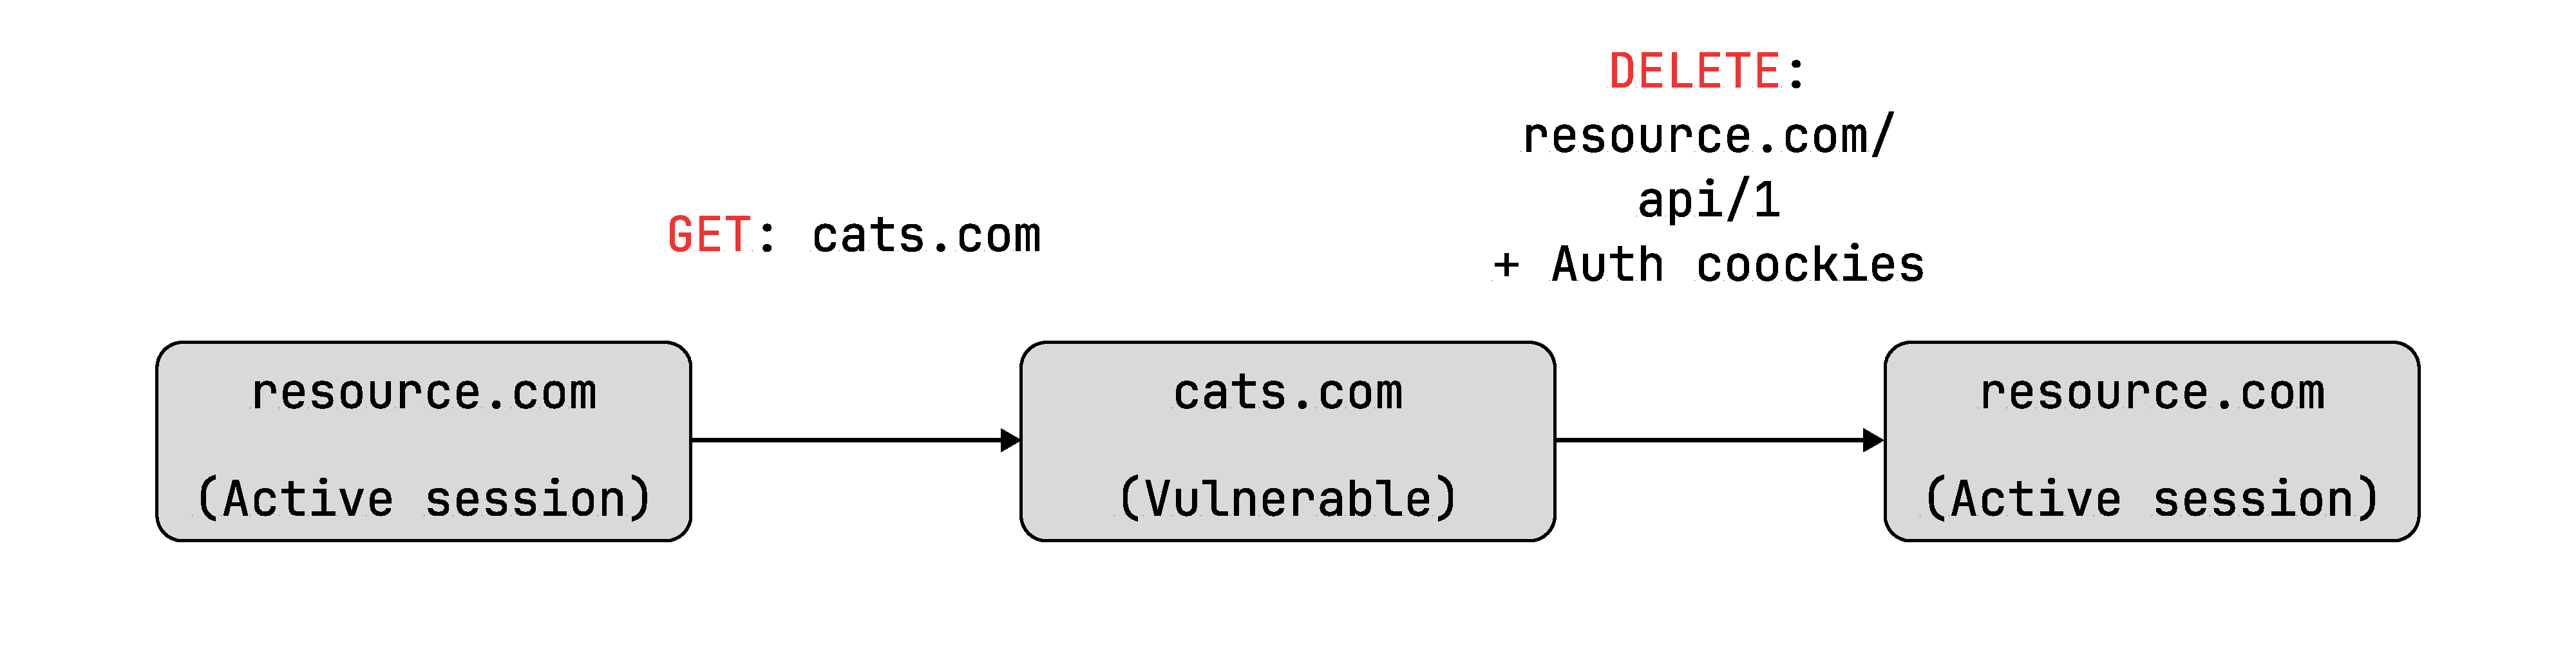
\includegraphics[width=1\textwidth]{img/Csrf_diagram}
    ~\caption{CSRF attack principle diagram.}\label{fig:csrf_diagram}
\end{figure}

Cookie files provided with \texttt{SameSite} setting that determines whether cookies will be sent
along with cross-domain requests.

\texttt{SameSite} setting has one of the states below:

\begin{itemize}
    \item \textbf{None} means no restrictions are imposed on the transfer of cookies.
    \item \textbf{Lax} allows cookie transmission only by secure HTTP methods, according to RFC 7231~\cite{fielding2014rfc}.
    These methods are \texttt{GET, HEAD, OPTIONS} and \texttt{TRACE}.
    \item \textbf{Strict} blocks cookies from being sent with any requests from third-party resources.
    Cookies will only be transferred within the same domain.
\end{itemize}

Therefore, \texttt{SameSite} setting values such as \texttt{Lax} and \texttt{Strict} protect user from a CSRF attack
blocking submission of cookies using unsecure HTTP methods and cross-domain requests.
There are more CSRF protection techniques in~\cite{owaspCsrf}.


    \section{Introduction} \label{sec:introduction}
    Your introduction here.
Include some references~\cite{siddiqui2011cross,spett2005cross, bradley2015rfc,hardt2012oauth}.
Lorem Ipsum is simply dummy text of the printing and typesetting industry.
Lorem Ipsum has been the industry's standard dummy text ever since the 1500s, when an unknown printer took a galley
of type and scrambled it to make a type specimen book.
It has survived not only five centuries, but also the leap into electronic typesetting, remaining essentially unchanged.
It was popularised in the 1960s with the release of Letraset sheets containing Lorem Ipsum passages, and more
recently with desktop publishing software like Aldus PageMaker including versions of Lorem Ipsum.

OAuth 2.0 flow diagram
\begin{figure}[H]
    \centering
    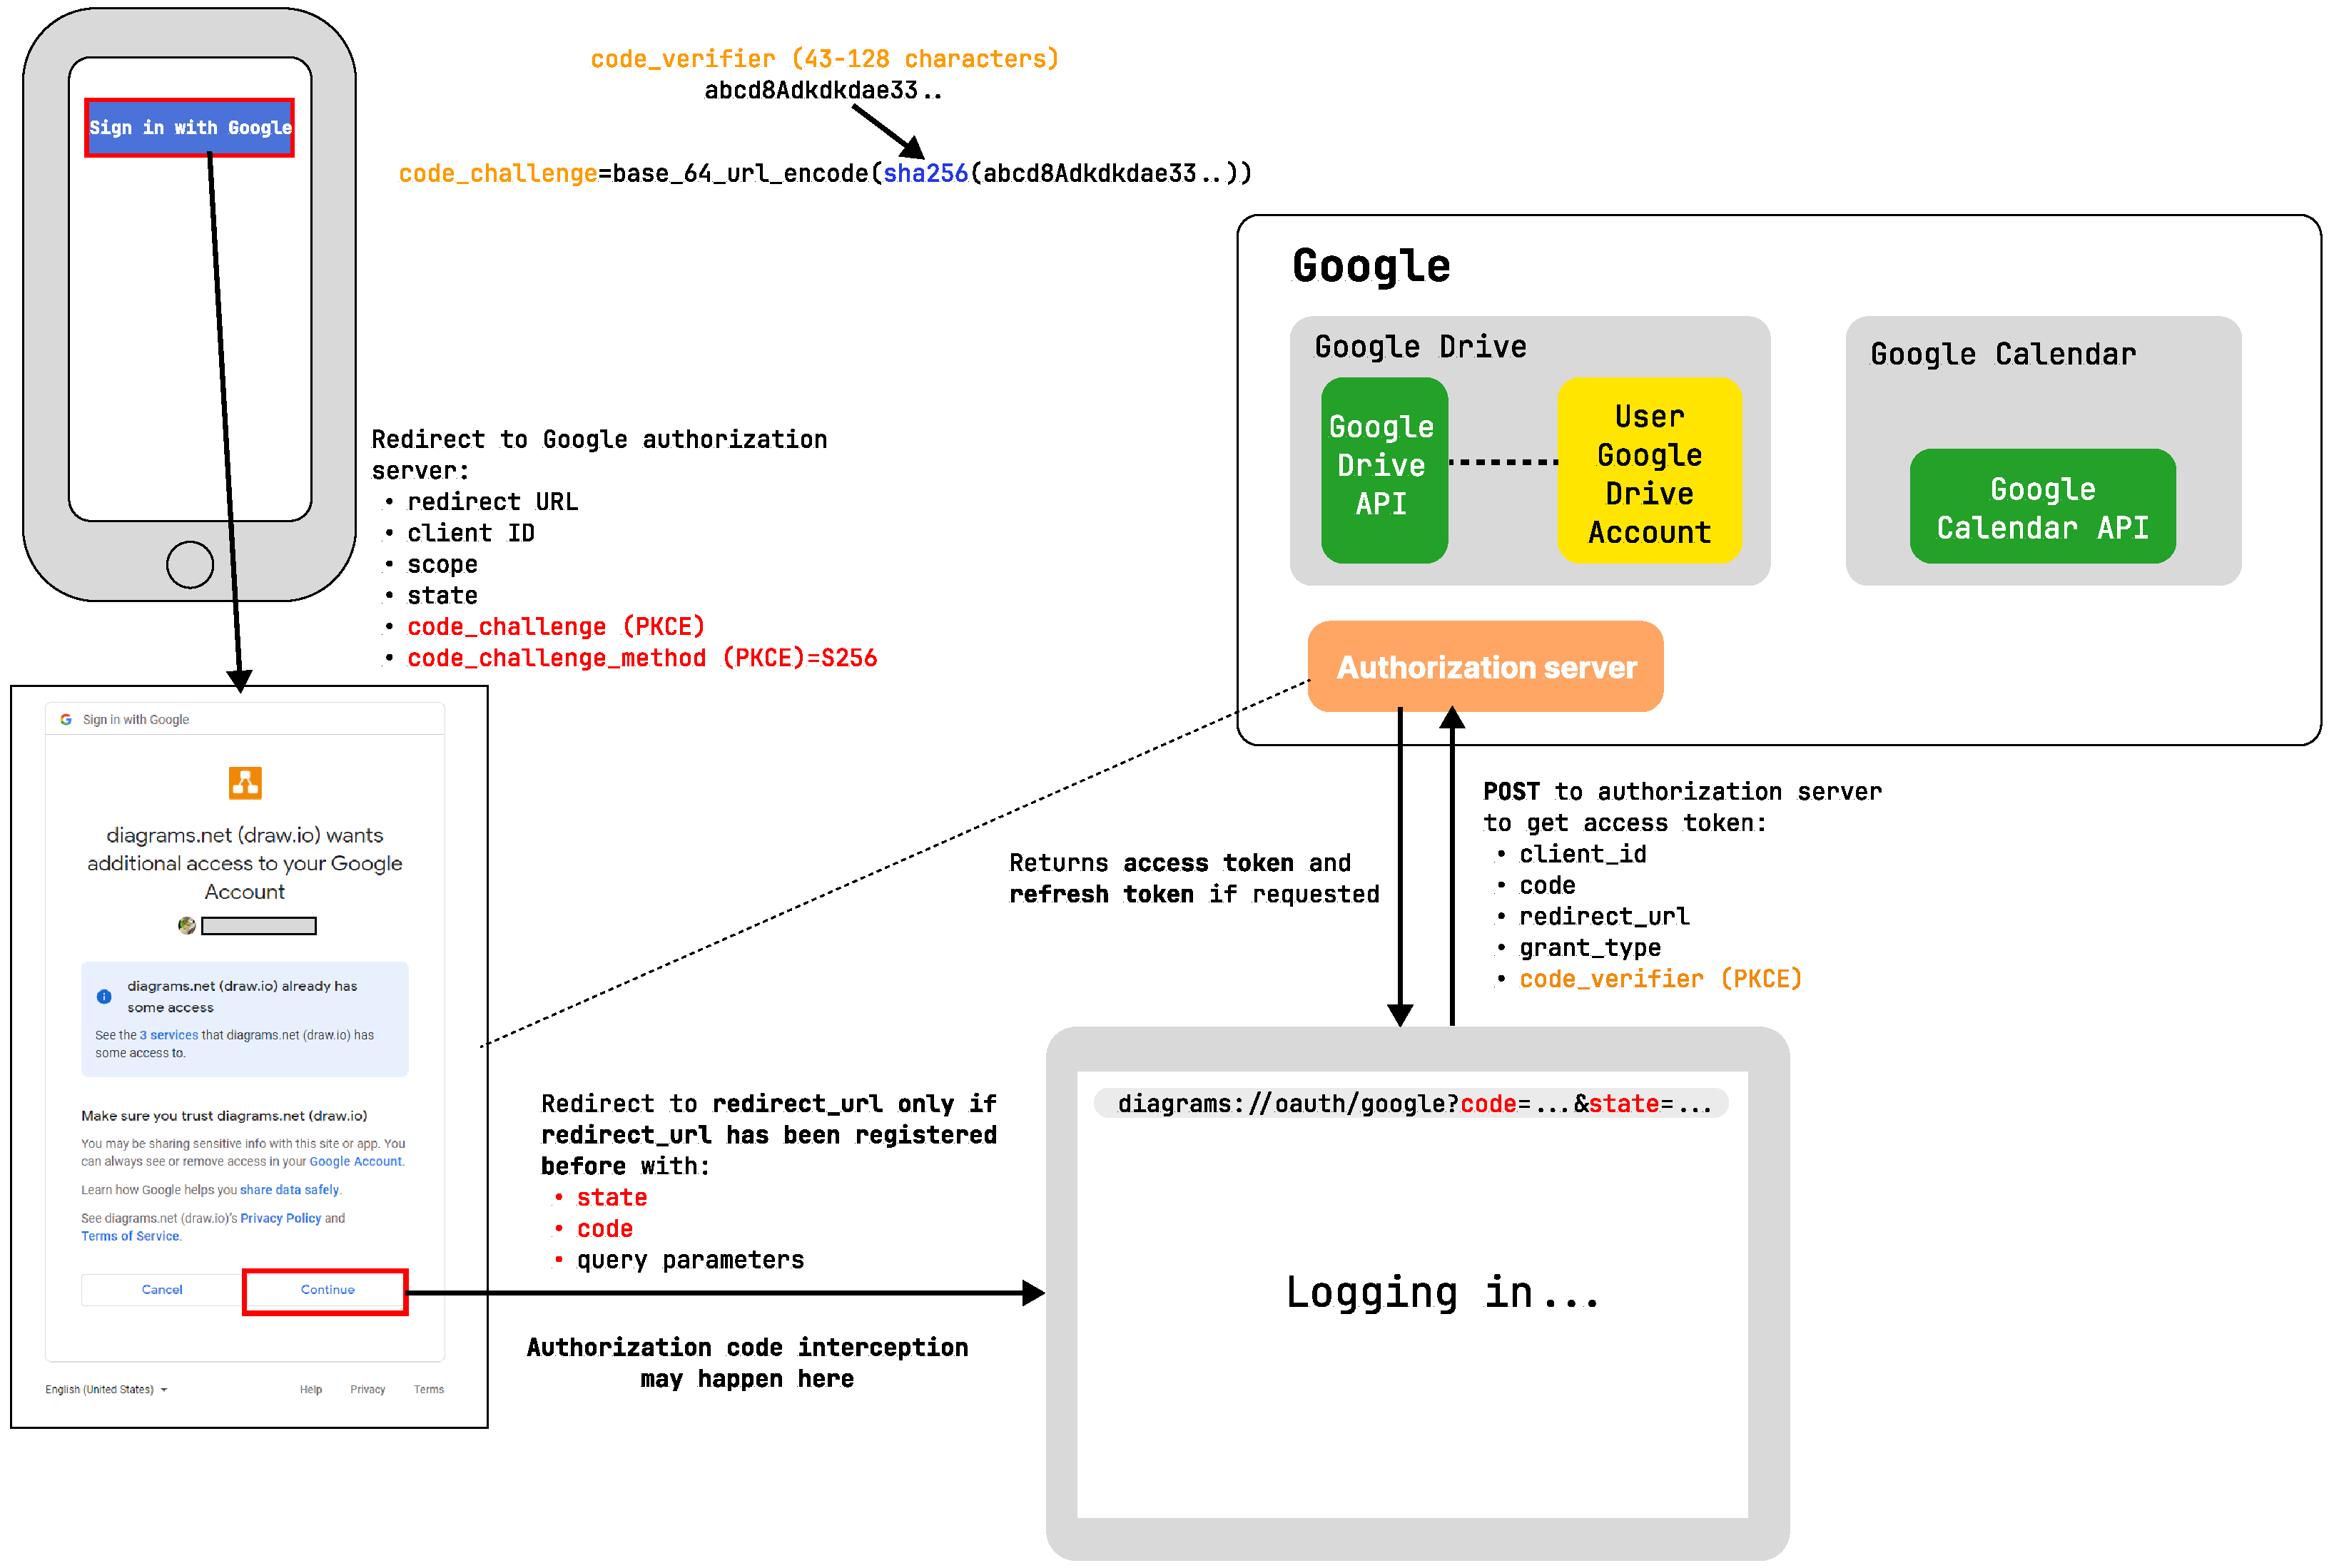
\includegraphics[width=1\textwidth]{img/OAuthPkceScheme_1570_1055}
    ~\caption{OAuth 2.0 with PKCE flow diagram.}\label{fig:oauth_with_pkce}
\end{figure}


    \section{Authentication flow}\label{sec:authentication-flow}
    Consider a more practical approach that takes all the previously discussed aspects.
Applying modern frameworks like ASP .NET Core, Angular etc.
let be the following authentication flow as per diagram below
\begin{figure}[H]
    \centering
    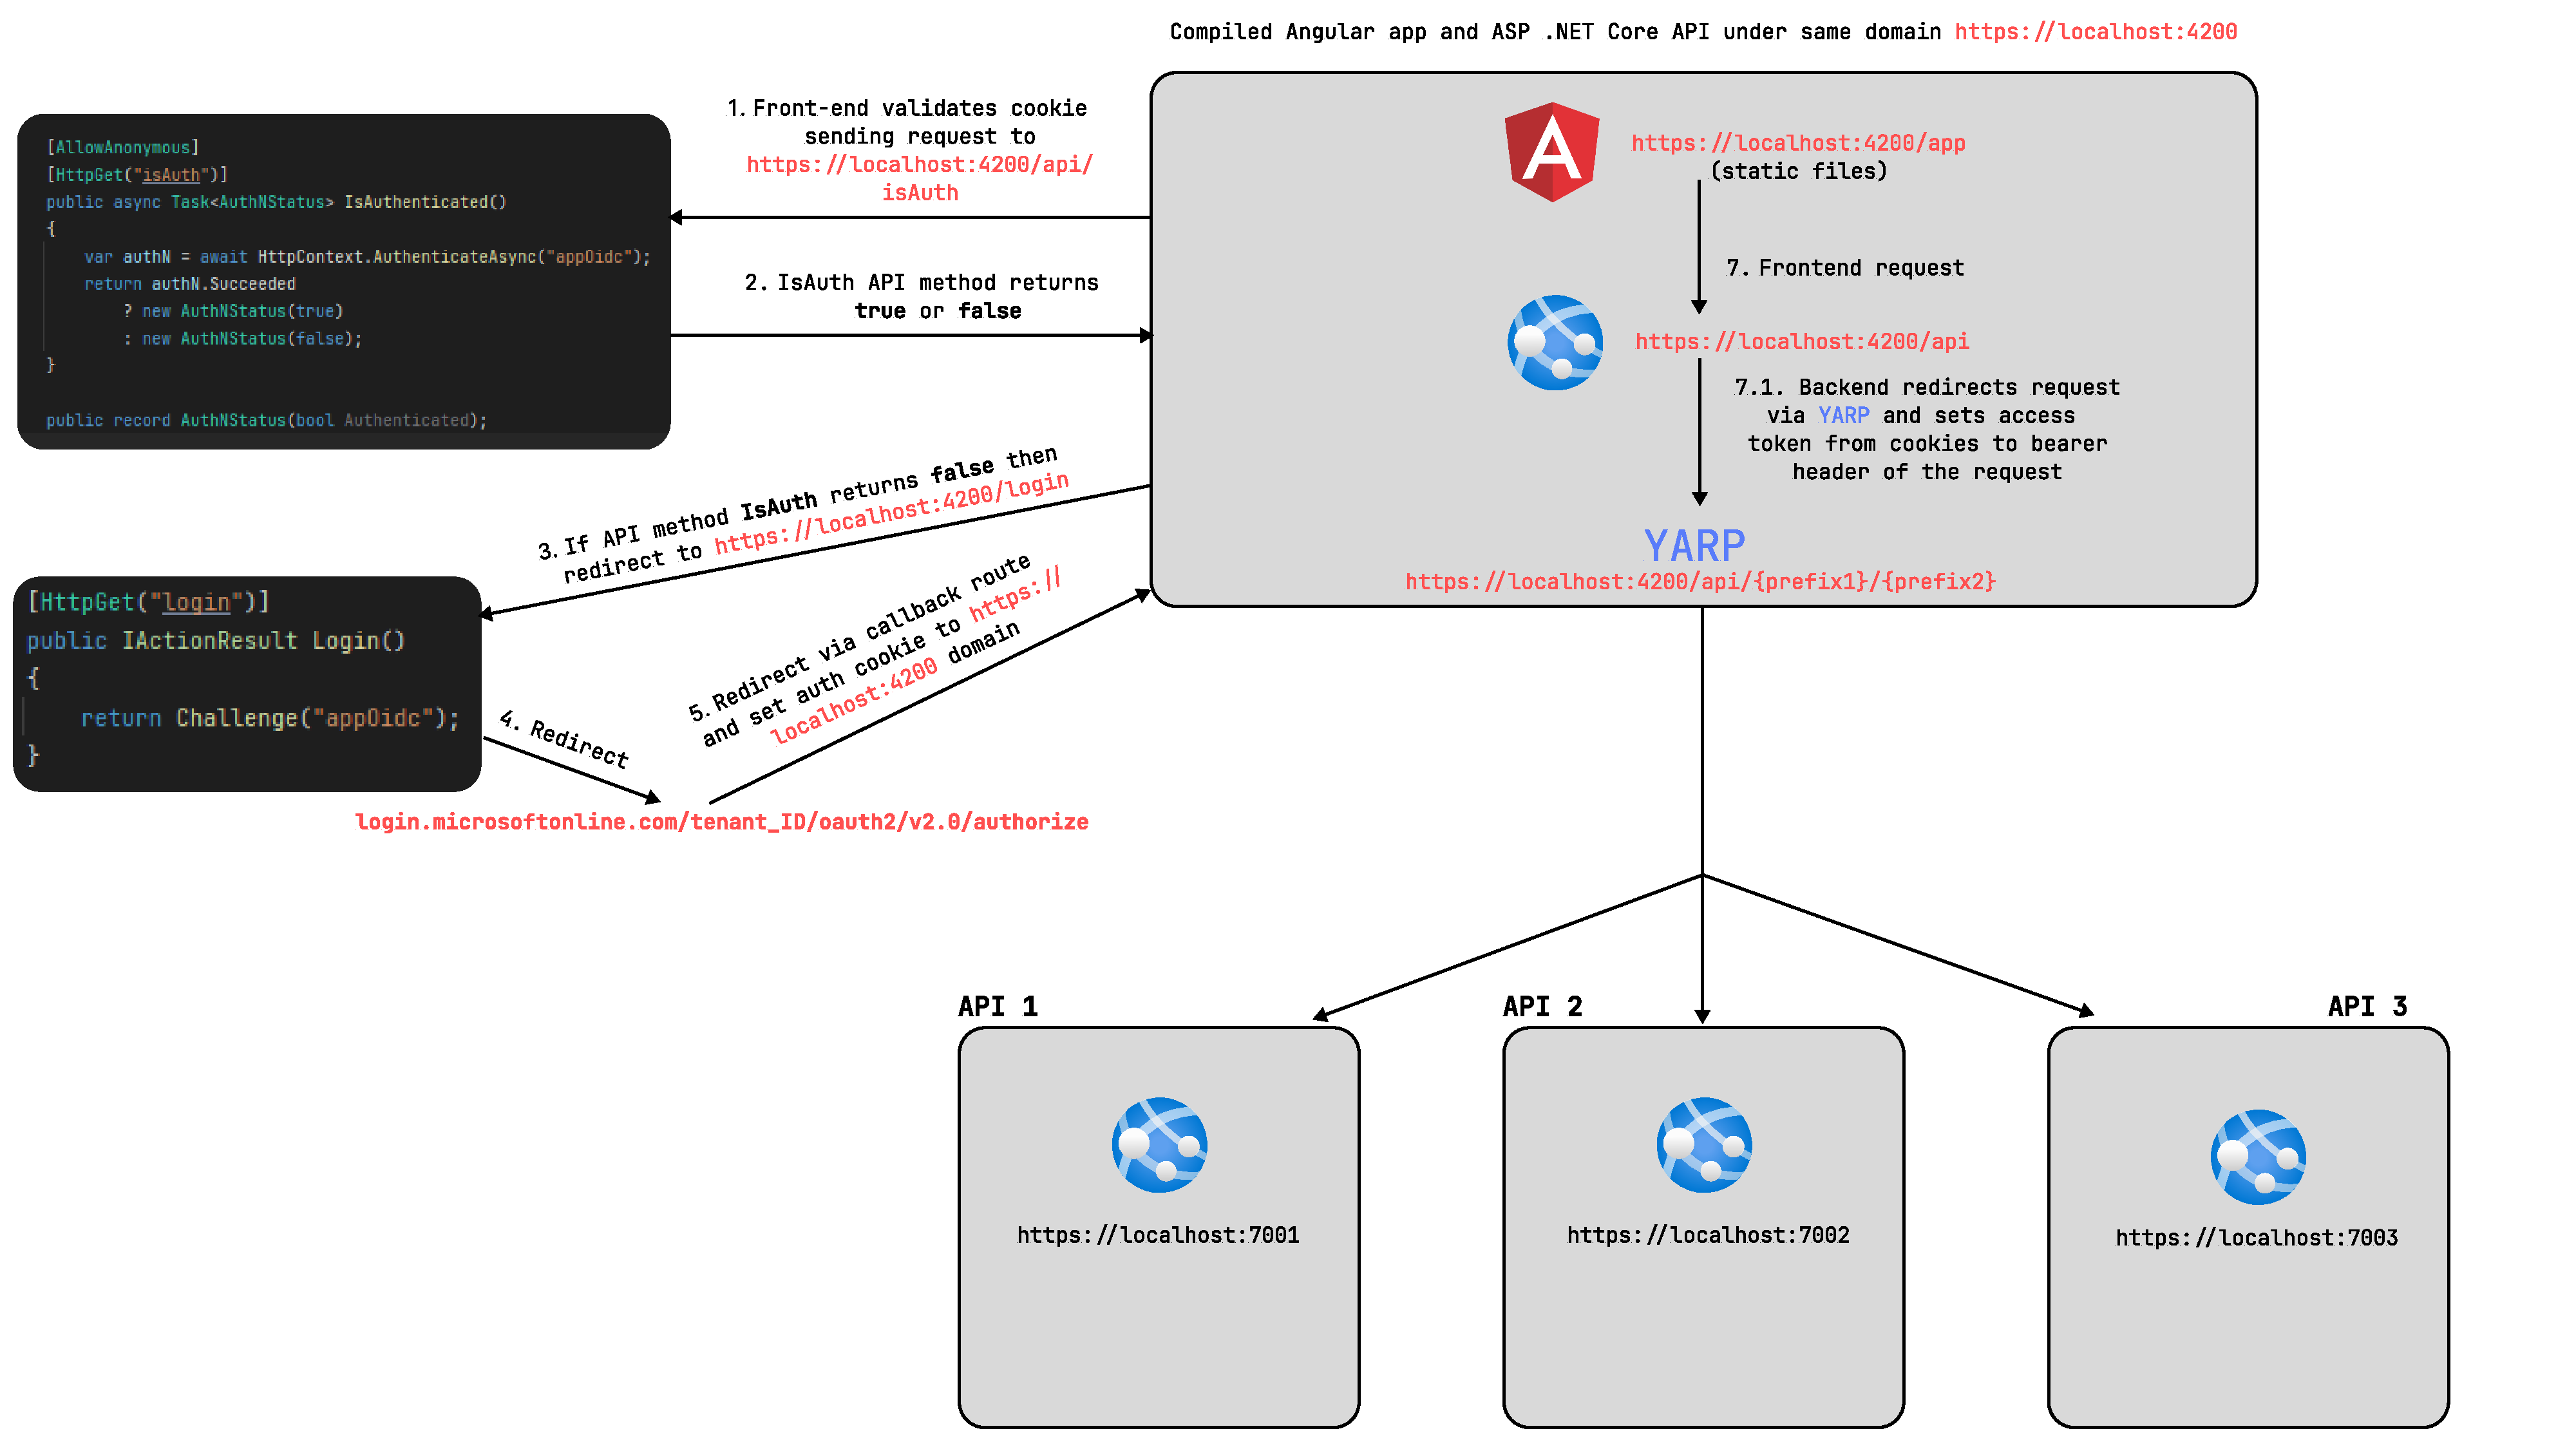
\includegraphics[width=1\textwidth]{img/Auth_flow_updated}
    ~\caption{Authentication flow diagram.}\label{fig:authentication_flow_diagram}
\end{figure}

Therefore, the whole authentication process can be described as eight steps such that
\begin{enumerate}
    \item Compiled Angular frontend application sends request to the authentication endpoint of the ASP .NET Core API
    to verify current authentication state.
    Angular application is a set of precompiled bundles that are exposed via same ASP .NET Core API at the \texttt{/app}
    endpoint so that cross-origin requests are not necessary and tokens can be stored in cookie files securely
    \item Authentication endpoint of the ASP .NET Core API responses either with
    HTTP status code \texttt{200 (OK)} or \texttt{401 (Unauthorized)}
    \item If \texttt{401 (Unauthorized)} status code received from previous step,
    then browser is redirected to the \texttt{login} endpoint of the ASP .NET Core API,
    otherwise user gets access to the protected resources
    \item Login method of the ASP .NET Core API redirects browser to the Azure AD authorize url
    \texttt{login.microsoftonline.com/tenant/oauth2/v2.0/authorize} where user enters his credentials.
    It is important to clarify that in order to get ID token we have to put parameter \texttt{openid} to the scope
    \begin{spverbatim}
    serviceCollection
    .AddAuthentication(options => {...})
    .AddCookie(CookieAuthenticationDefaults.AuthenticationScheme, options => {...})
    .AddOpenIdConnect(AuthConstants.AppOidc, options =>
        {
        ...
        options.Scope.Add("openid");
    });
\end{spverbatim}
    \item After successful authentication on the Azure AD side, the browser is redirected to the \texttt{fallback\_url}
    that is defined in Azure AD application registration.
    This \texttt{fallback\_url} is an active endpoint of the ASP .NET Core API\@.
    At this point, the \texttt{TickerStore}~\cite{microsoftIticketstore2023, ticketStore_2023}
    comes into the flow to manage user sessions.
    Each session is stored as a \texttt{UserSessionEntity} entity in the database.
    \begin{spverbatim}
    public class UserSessionEntity
    {
        public Guid Id { get; set; }
        public DateTimeOffset CreatedAt { get; set; }
        public DateTimeOffset ExpiresAt { get; set; }
        public DateTimeOffset UpdatedAt { get; set; }
        public DateTimeOffset DateOfLastAccess { get; set; }
        public byte[] Value { get; set; }
    }
\end{spverbatim}
    The Value property of type \texttt{byte[]} contains serialized \texttt{AuthenticationTicket}~\cite{microsoftAuthenticationTicket2023}
    object such that contains all required information like access, ID and refresh tokens.
    The class \texttt{TickerStore} implements \texttt{ITickerStore} interface that offers 4 methods:
    \texttt{StoreAsync, RenewAsync, RetrieveAsync, RemoveAsync}.
    \begin{itemize}
        \item The \texttt{StoreAsync} method is executed immediately after authentication on the authentication server,
        it saves the user session to the database.
        \item The \texttt{RenewAsync} method in our case is used by the background service to update user sessions.
        \item The \texttt{RetrieveAsync} method is executed every time a request is sent to the endpoint marked with the
        \texttt{[Authorize]} attribute.
        \item The \texttt{RemoveAsync} method is executed when the browser cookie has expired,
        as well as is used by the same \texttt{RefreshBackgroundService}
        to remove sessions which have not been used for a long time.
    \end{itemize}
    Example \texttt{TicketStore} implementation can be found at~\cite{ticketStore_2023}.
    Example of \texttt{TicketStore} dependency injection can be found at~\cite{ticketStoreDI_2023}.
    Authentication cookies are being setup at this step.
    \item Step 1 is repeated here, but now the HTTP request is for sure to be with \texttt{200 (OK)} status code.
    \item Precompiled Angular frontend application now sends request to the another microservice with authentication cookies
    attached to the request's \texttt{Bearer} header using YARP library~\cite{microsoftYarp2021, yarpSectionAppSettings_2023},
    so that microservice is accessible.
    \item If previous step returns \texttt{401 (Unauthorized)} status code, then Step 1 is repeated
\end{enumerate}


    \section{Refresh token flow}\label{sec:refresh-token-flow}
    The implementation of refreshing user tokens is extremely simple.
It is necessary to create a background service~\cite{microsoftHostedservice2023} that manages sessions,
in particular deletes sessions that have not been used long time, refresh existing sessions, etc.
In case of refresh or initial authentication, the new \texttt{AuthenticationTicket} object~\cite{microsoftAuthenticationTicket2023}
replaces the existing or new instance is created.
In addition, the Azure AD authentication server's response contains a timestamp property \texttt{ExpiresIn}
that determines the lifetime of the tokens,
the background service updates the \texttt{ExpiresAt} property of the \texttt{UserSessionEntity} accordingly.

The background service is responsible not only for refreshing the sessions,
but also it is responsible for deleting the sessions that have not been used for a long time.
Once per predefined period, the sessions are selected and their \texttt{DateOfLastAccess} property is
compared to the current \texttt{DateTime.Now}.
If the difference between the \texttt{DateOfLastAccess} and \texttt{DateTime.Now} is more than, for example, 3 days,
 then the session is deleted.
Each time a user performs an action on the site, the \texttt{DateOfLastAccess} property is updated.
Implementation of a background service can be done as per references~\cite{backroundService_2023, configurationBackgroundService_2023}


    \section{Conclusions}\label{sec:conclusions}
    In this manuscript we explore the problem of secure storage and transfer of access tokens between microservices.
Particular attention was paid to possible vulnerabilities during transfer of access tokens such
as Cross-Site Scripting (XSS) and Cross-Site Request Forgery (CSRF).

To eliminate these vulnerabilities, it is necessary to store authorization tokens in cookies with mandatory
\texttt{HttpOnly} and \texttt{SameSite} settings such that \texttt{SameSite} values should be \texttt{Lax} or \texttt{Strict}.
Therefore, cookies are either transmitted via secure \texttt{HTTP} methods or not transmitted at all.

User authentication to be implemented using the OIDC protocol~\cite{siriwardenaOpenid2020, sakimuraOpenid2014}
in couple with Authorization code flow with PKCE~\cite{bradley2015rfc}.
The main principle of the OIDC protocol is described more detailed in Chapter 2.

Also, we provide an authentication / authorization implementation based on the ASP.NET Core Web API backend and Angular
frontend application.
These apps are stored under single domain to eliminate necessity to transfer authorization cookies cross domain way.
The transfer of access tokens to microservices is implemented using Reverse Proxy YARP~\cite{microsoftYarp2021} so that
the access token is automatically substituted in the request header.

In addition, we proposed a mechanism to refresh an access token through the Ticket Store~\cite{microsoftIticketstore2023} entity
and Hosted Service~\cite{microsoftHostedservice2023}.
Therefore, the Ticket Store checks each request for access token expiration.
In case of expiration of the access token, the access token is refreshed by means of authorization microservice.
Ticket store also stores the pair of the access and refresh token inside \texttt{AuthenticationTicket} entity~\cite{microsoftAuthenticationTicket2023}.

Finally, in this manuscript we proposed a solution to the problem of securely storing an access token and passing it between microservices,
eliminating the Cross-Site Scripting (XSS) and Cross-Site Request Forgery (CSRF) vulnerabilities.


    \section{Acknowledgements}\label{sec:acknowledgements}
    Thanks someone and somebody for help and useful comments.

    \bibliographystyle{unsrt}
    \bibliography{SecureAzureOIDCReferences}

\end{document}
